% Adjust these for the path of the theme and its graphics, relative to this file
%\usepackage{beamerthemeFalmouthGamesAcademy}
\usepackage{../../beamerthemeFalmouthGamesAcademy}
\usepackage[utf8]{inputenc}
\usepackage{multimedia}
\graphicspath{ {../../} }

% Default language for code listings
\lstset{language=Python
}

% For strikethrough effect
\usepackage[normalem]{ulem}
\usepackage{wasysym}

\usepackage{algpseudocode}

\usepackage{pdfpages}

% http://www.texample.net/tikz/examples/state-machine/
\usetikzlibrary{arrows,automata}

\newcommand{\modulecode}{COMP702}\newcommand{\moduletitle}{Classical Artificial Intelligence}\newcommand{\sessionnumber}{1}

\begin{document}
\title{\sessionnumber: Flowcharts and pseudocode}
\subtitle{\modulecode: \moduletitle}

\frame{\titlepage} 

\begin{frame}
	\frametitle{Learning outcomes}
	\begin{itemize}
		\item Explain and use basic data types
		\item Recall some basic algorithms
		\item Produce and explain basic flowcharts
		\item Produce and explain basic pseudocode
	\end{itemize}
\end{frame}

\part{Data types}
\frame{\partpage}

\begin{frame}{What is a type?}
	\begin{itemize}
		\pause\item A \textbf{variable} in Python holds a \textbf{value}
		\pause\item Every value has a \textbf{type}
		\pause\item The type of a value dictates:
			\begin{itemize}
				\pause\item What sort of data it can hold
				\pause\item How the data is stored in memory
				\pause\item What operations can be done on it
			\end{itemize}
		\pause\item Python is \textbf{weakly typed} --- a variable can hold a value of any type
		\pause\item Many languages are \textbf{strongly typed} --- a variable has a defined type and can only hold values of that type
	\end{itemize}
\end{frame}

\begin{frame}{Memory}
	\pause
	\begin{center}
		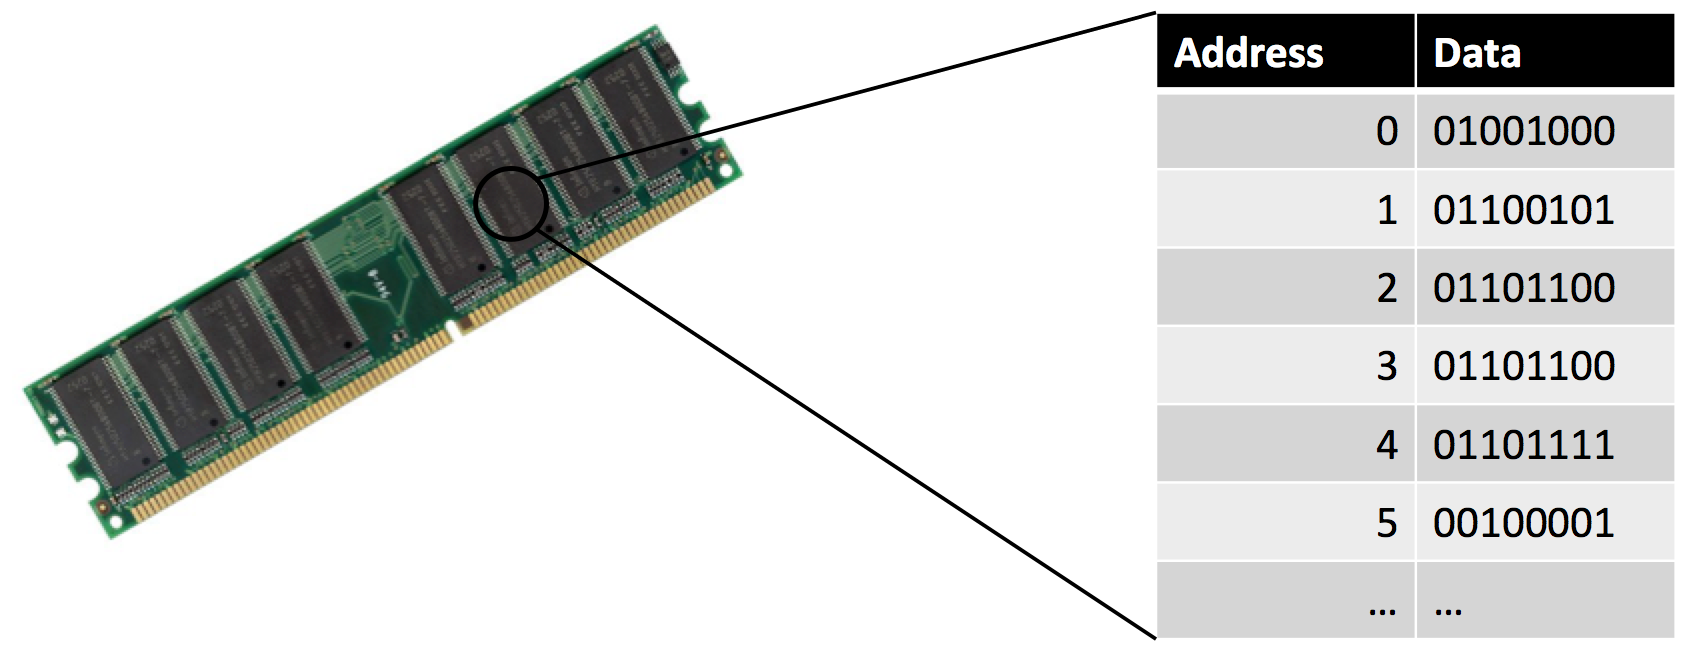
\includegraphics[width=0.8\textwidth]{memory}
	\end{center}
	\begin{itemize}
		\item Memory works like a set of \textbf{boxes}
		\pause\item Each box has a number, its \textbf{address}
		\pause\item Each box contains a \textbf{byte} (8 bits)
	\end{itemize}
\end{frame}

\begin{frame}{Data representation} 
	\begin{itemize}
		\pause\item All data is stored as \textbf{sequences of bytes}
			\begin{itemize}
				\pause\item Sequence of bits, in multiples of 8
				\pause\item Sequence of numbers between 0--255
			\end{itemize}
	\end{itemize}
\end{frame}

\begin{frame}{Integers}
	\begin{itemize}
		\pause\item An \textbf{integer} is a whole number --- positive, negative or zero
		\pause\item Python type: \lstinline{int}
		\pause\item In most languages, \lstinline{int} is limited to 32 or 64 bits
		\pause\item Python uses \textbf{big integers} --- number of bits expands automatically to fit the value to be stored
		\pause\item Stored in memory using binary notation, with 2's complement for negative values
	\end{itemize}
\end{frame}

\begin{frame}{Floating point numbers}
	\begin{itemize}
		\pause\item What about storing non-integer numbers?
		\pause\item Usually we use \textbf{floating point} numbers
		\pause\item Python type: \lstinline{float}
		\pause\item Details on in-memory representation later in the module
		\pause\item (Note: \lstinline{float} in Python 3 has the same precision as \lstinline{double} in C++/C\#/etc)
	\end{itemize}
\end{frame}

\begin{frame}{Integers vs floating point numbers}
	\begin{itemize}
		\pause\item \lstinline{int} and \lstinline{float} are different types!
		\pause\item \lstinline{42} and \lstinline{42.0} are technically different values
			\begin{itemize}
				\pause\item One is an \lstinline{int}, the other is a \lstinline{float}
				\pause\item They are stored differently in memory
				\pause\item However \lstinline{==} etc still know how to compare them sensibly
			\end{itemize}
	\end{itemize}
\end{frame}

\begin{frame}{Booleans}
	\begin{itemize}
		\pause\item A \textbf{boolean} can have one of two values: \textbf{true} or \textbf{false}
		\pause\item Python type: \lstinline{bool}
		\pause\item In Python, we have the keywords \lstinline{True} and \lstinline{False}
		\pause\item Could be represented by a single bit in memory...
		\pause\item ... but since memory is addressed in bytes (or words of multiple bytes),
			usually represented as an \lstinline{int} with $0$ meaning \lstinline{False}
			and any non-zero (e.g.\ $1$) meaning \lstinline{True}
	\end{itemize}
\end{frame}

\begin{frame}[fragile]{Boolean values}
	\begin{itemize}
		\pause\item The \lstinline{if} statement takes a boolean value as its condition:
	\end{itemize}
	\begin{lstlisting}
if x > 10:
    print(x)
	\end{lstlisting}
	\begin{itemize}
		\pause\item Variables can also store boolean values:
	\end{itemize}
	\begin{lstlisting}
result = (x > 10)   # result now stores True or False
if result:
    print(x)
	\end{lstlisting}
\end{frame}

\begin{frame}{The ``None'' value}
	\begin{itemize}
		\pause\item Python has a special value \lstinline{None} which can be used to denote the ``absence'' of any other value
		\pause\item Python type: \lstinline{NoneType}
	\end{itemize}
\end{frame}

\begin{frame}{Strings}
	\begin{itemize}
		\pause\item A \textbf{string} represents a sequence of textual characters
		\pause\item E.g.\ \lstinline{"Hello world!"}
		\pause\item Python type: \lstinline{str}
	\end{itemize}
\end{frame}

\begin{frame}{Strings}
	\begin{itemize}
		\pause\item Stored as sequences of \textbf{characters} encoded as \textbf{integers}
		\pause\item Often \textbf{null-terminated}
			\begin{itemize}
				\pause\item Character number 0 signifies the end of the string
			\end{itemize}
		\pause\item \textbf{ASCII} encodes characters as 8-bit integers
			\begin{itemize}
				\pause\item 255 characters: Latin alphabet, numerals, punctuation
			\end{itemize}
		\pause\item \textbf{UTF-32} encodes characters as 32-bit integers
			\begin{itemize}
				\pause\item \textbf{Unicode} characters: ASCII + several other alphabets, Asian languages, symbols, emoji, ...
			\end{itemize}
		\pause\item \textbf{UTF-8} encodes characters as 8, 16, 24 or 32-bit integers
			\begin{itemize}
				\pause\item More common Unicode characters are smaller $\implies$ more efficient than UTF-32
			\end{itemize}
	\end{itemize}
\end{frame}

{
\setbeamercolor{background canvas}{bg=white}
\begin{frame}[plain]
	\begin{tikzpicture}[remember picture, overlay]
		\node[at=(current page.center)] {
			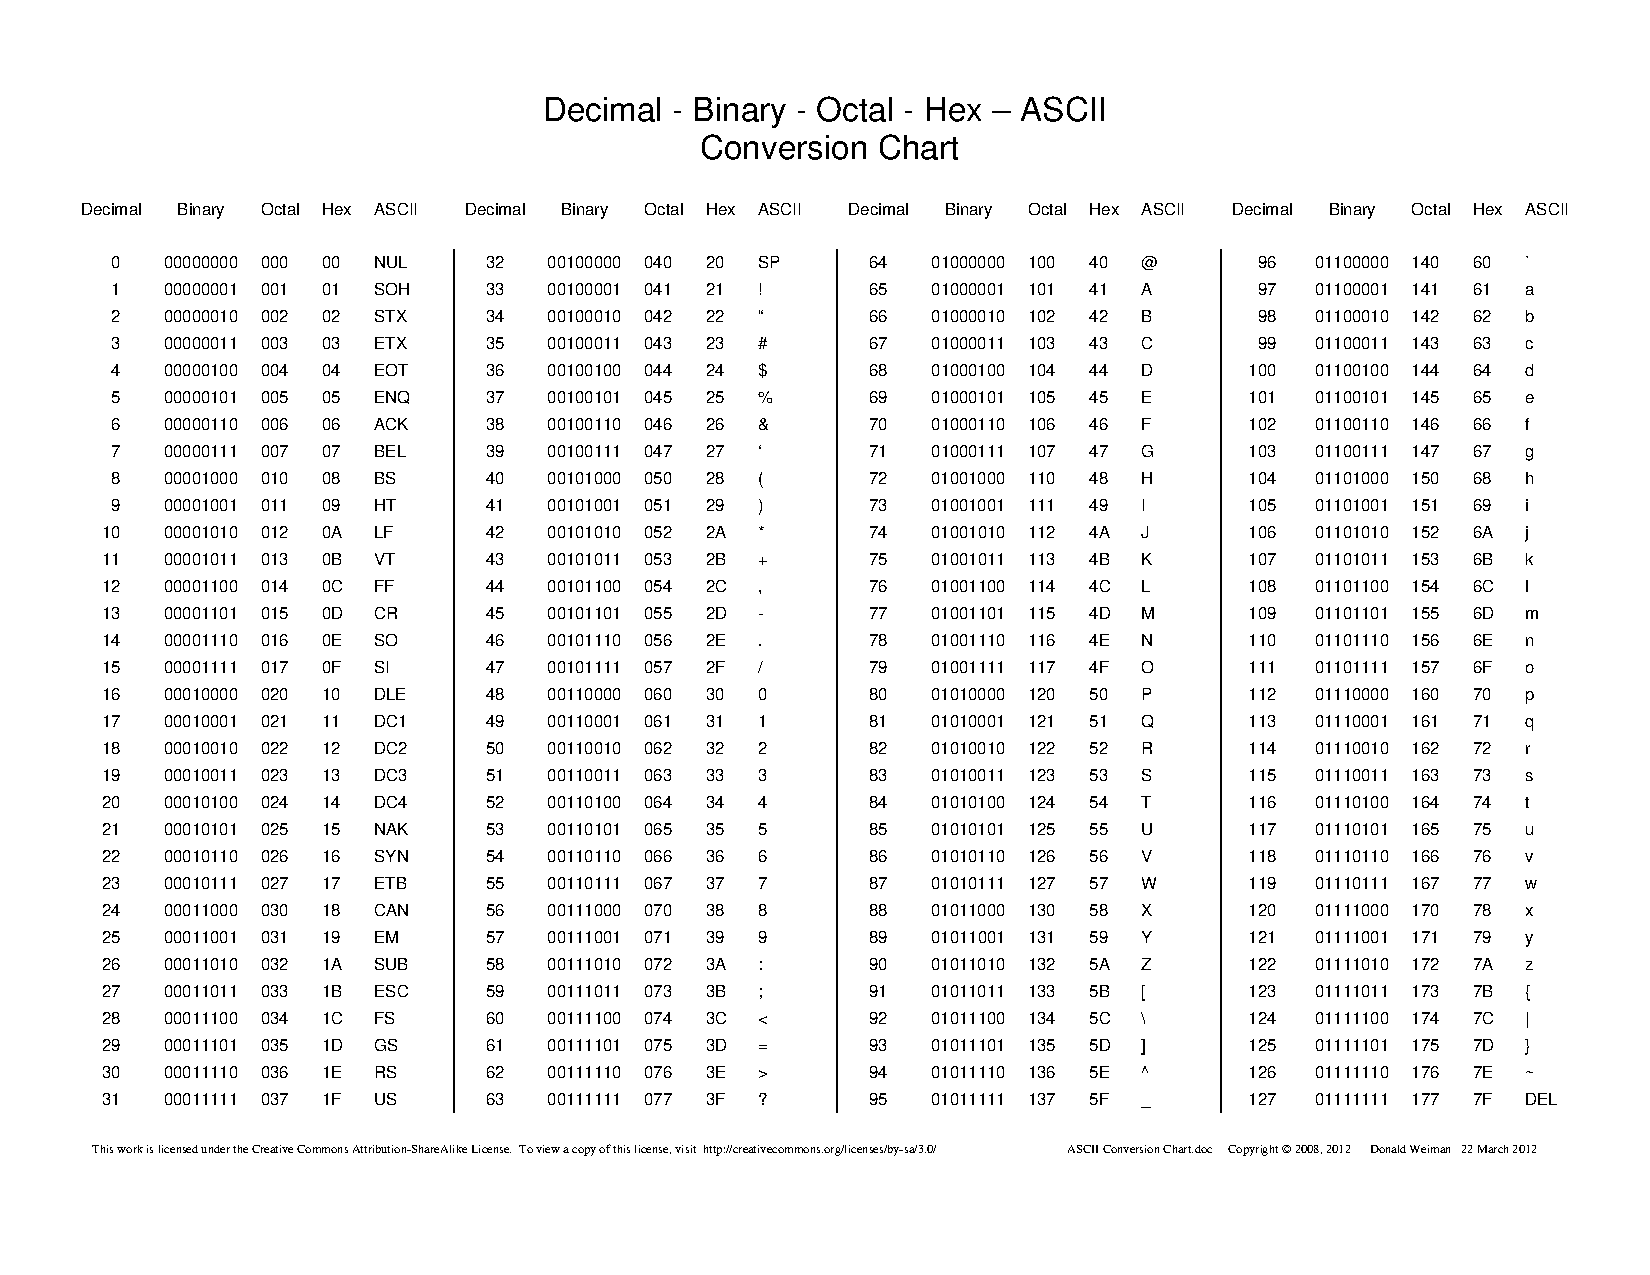
\includegraphics[width=\paperwidth]{ascii_chart}
		};
	\end{tikzpicture}
\end{frame}
}

\begin{frame}{String representation}
	\begin{itemize}
		\pause\item \lstinline{"Hello world!"} in ASCII encoding:
	\end{itemize}
	
	{\footnotesize\pause\begin{tabular}{*{13}{|c}|}
		\hline
		72 & 101 & 108 & 108 & 111 & 32 & 119 & 111 & 114 & 108 & 100 & 33 & 0 \\\hline
	\end{tabular}}
\end{frame}

\begin{frame}{UTF-8 representation}
	\begin{itemize}
		\pause\item For characters in ASCII, UTF-8 is the same:
			\begin{itemize}
				\pause\item a $\to [97]$
			\end{itemize}
		\pause\item Other characters are encoded as multi-byte sequences:
			\begin{itemize}
				\pause\item \"u $\to [195, 188]$
				\pause\item 
\includegraphics[height=1.5ex]{chinese}\ $\to [228, 184, 178]$
				\pause\item 
\includegraphics[height=1.5ex]{emoji}\ $\to [240, 159, 152, 130]$
			\end{itemize}
	\end{itemize}
\end{frame}

\begin{frame}{Type casting}
	\begin{itemize}
		\pause\item It is often useful to \textbf{cast}, or \textbf{convert}, a value from one type to another
		\pause\item In Python, this is done by calling the type as if it were a function
			\begin{itemize}
				\pause\item \lstinline{float(17)} $\to$ \lstinline{17.0}
				\pause\item \lstinline{int(3.14)} $\to$ \lstinline{3}
				\pause\item \lstinline{str(3.14)} $\to$ \lstinline{"3.14"}
				\pause\item \lstinline{str(1 + 1 == 2)} $\to$ \lstinline{"True"}
				\pause\item \lstinline{int("123")} $\to$ \lstinline{123}
				\pause\item \lstinline{int("five")} gives an error
			\end{itemize}
	\end{itemize}
\end{frame}

\begin{frame}{Other types}
	\begin{itemize}
		\pause\item \textbf{Container} types for collecting several values
			\begin{itemize}
				\pause\item \lstinline{list}, \lstinline{tuple}, \lstinline{dict}, \lstinline{set}, ...
			\end{itemize}
		\pause\item \textbf{Objects}
		\pause\item Almost everything in Python is a value with a type
			\begin{itemize}
				\pause\item Functions, modules, classes, exceptions, ...
				\pause\item Even types themselves are values of type \lstinline{type}!
			\end{itemize}
	\end{itemize}
\end{frame}


\part{Algorithms}
\frame{\partpage}

\begin{frame}{What is an algorithm?}
	\pause\begin{center}
		A \textbf{sequence of instructions} which can be followed \textbf{step by step}
		to perform a \textbf{computational task}.
	\end{center}
\end{frame}

\begin{frame}{Programs vs algorithms}
	\begin{itemize}
		\pause\item A program is \textbf{specific} to a particular programming language and/or machine
		\pause\item An algorithm is \textbf{general}
		\pause\item An algorithm must be \textbf{implemented} as a program before a computer can run it
		\pause\item An algorithm generally performs \textbf{one task}, whereas a program may perform \textbf{many}
		\begin{itemize}
			\pause\item E.g.\ Microsoft Word is not an algorithm, but it implements many algorithms
			\pause\item E.g.\ it implements an algorithm for determining where to break a line of text,
				how much space to add to centre a line, etc.
		\end{itemize}
	\end{itemize}
\end{frame}

\begin{frame}{Algorithms outside computing}
	\begin{center}
		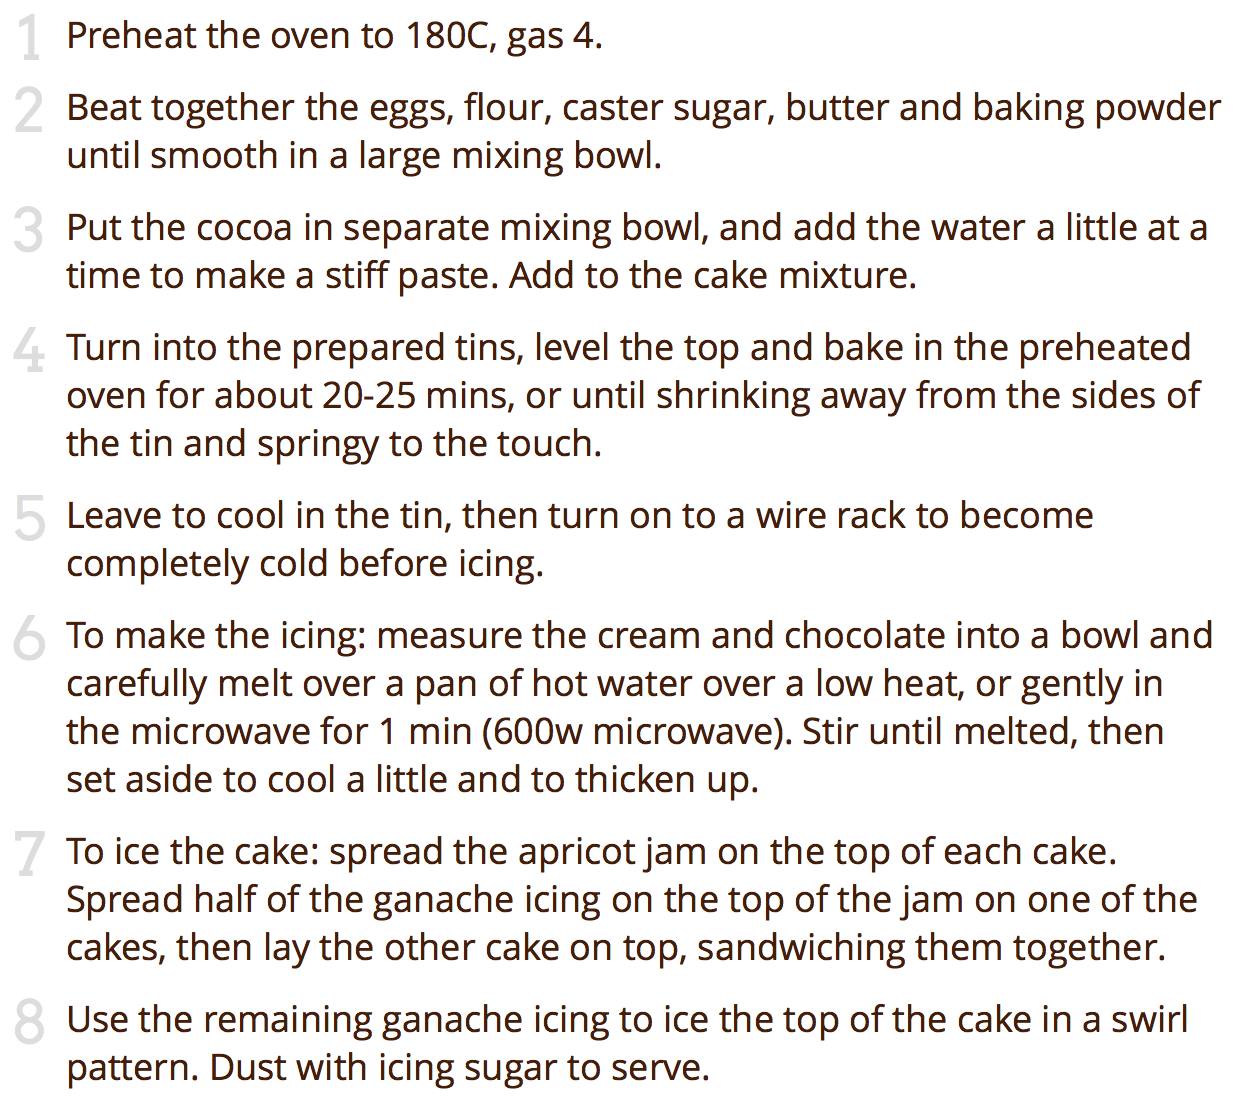
\includegraphics[height=0.8\textheight]{cake_recipe}
	\end{center}
\end{frame}

\begin{frame}{Algorithms outside computing}
	\begin{center}
		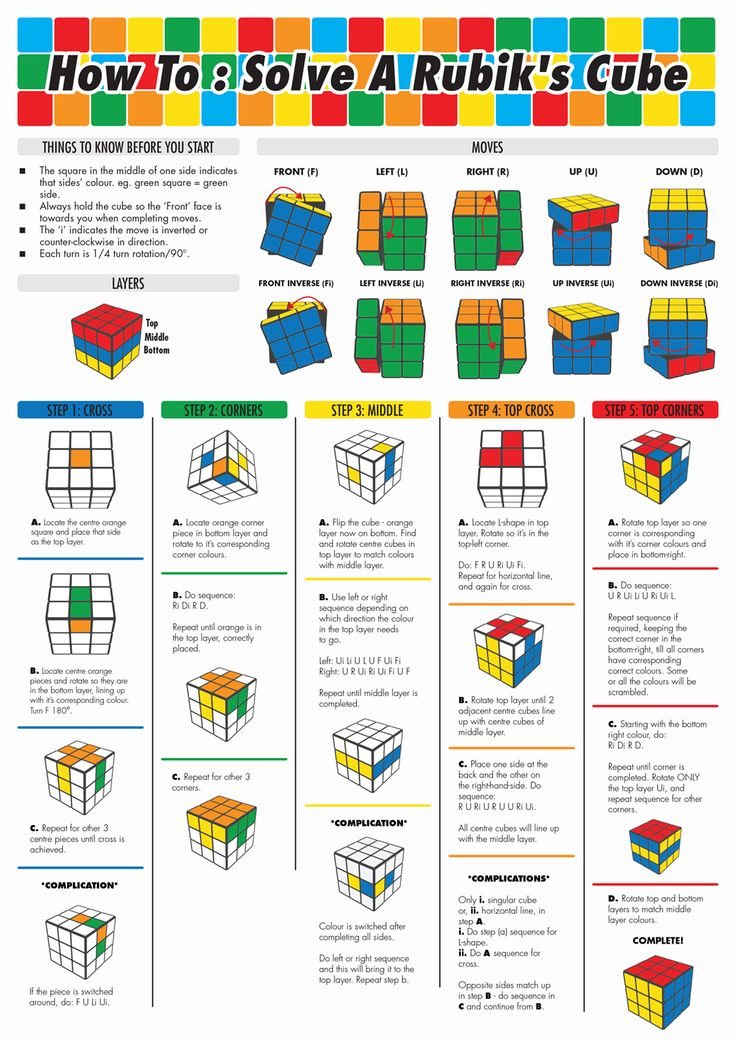
\includegraphics[height=0.8\textheight]{rubik_algorithm}
	\end{center}
\end{frame}

\part{Flowcharts}
\frame{\partpage}

\begin{frame}
	\begin{center}
		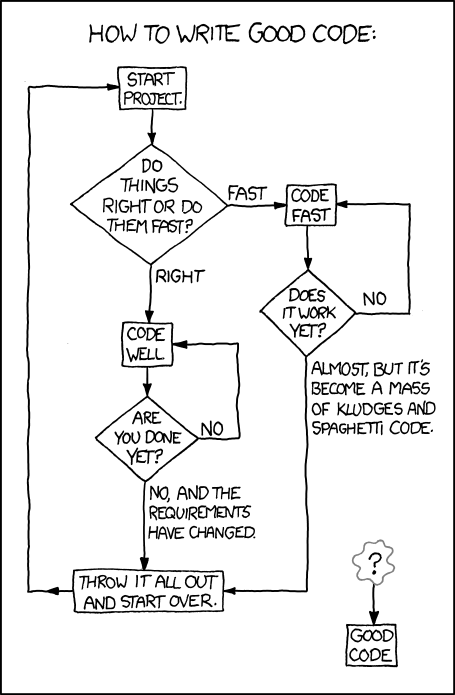
\includegraphics[height=0.9\textheight]{xkcd_good_code}
		
		{\tiny\url{http://xkcd.com/844/}}
	\end{center}
\end{frame}

\begin{frame}{Flowchart symbols}
	\begin{center}
		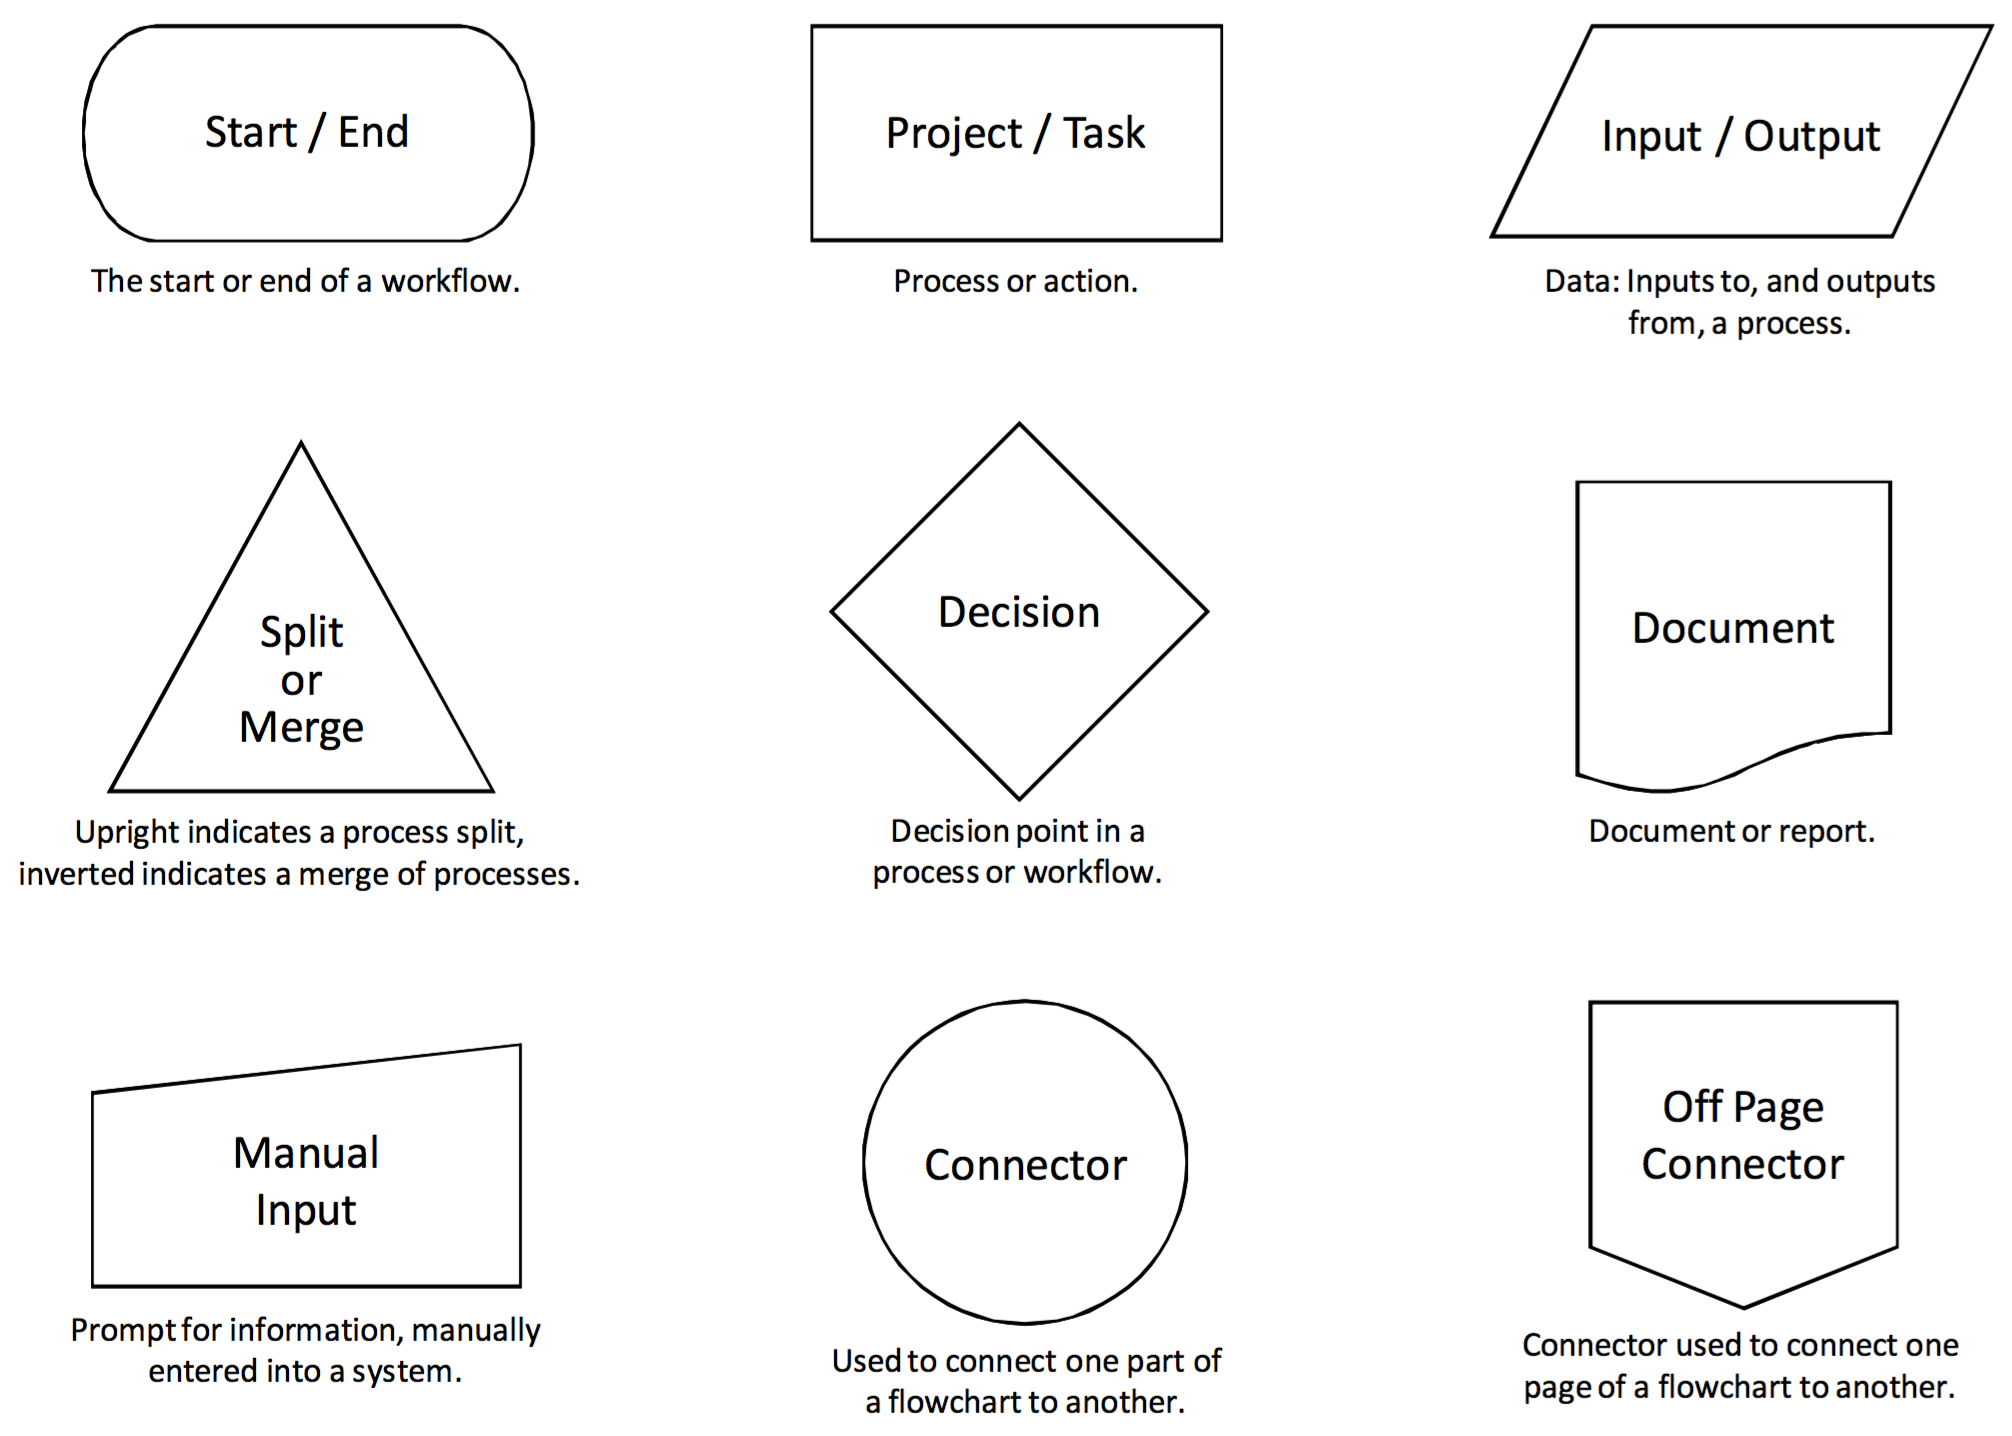
\includegraphics[height=0.8\textheight]{flowchart_symbols}
	\end{center}
\end{frame}

\begin{frame}{Swimlanes}
	\begin{center}
		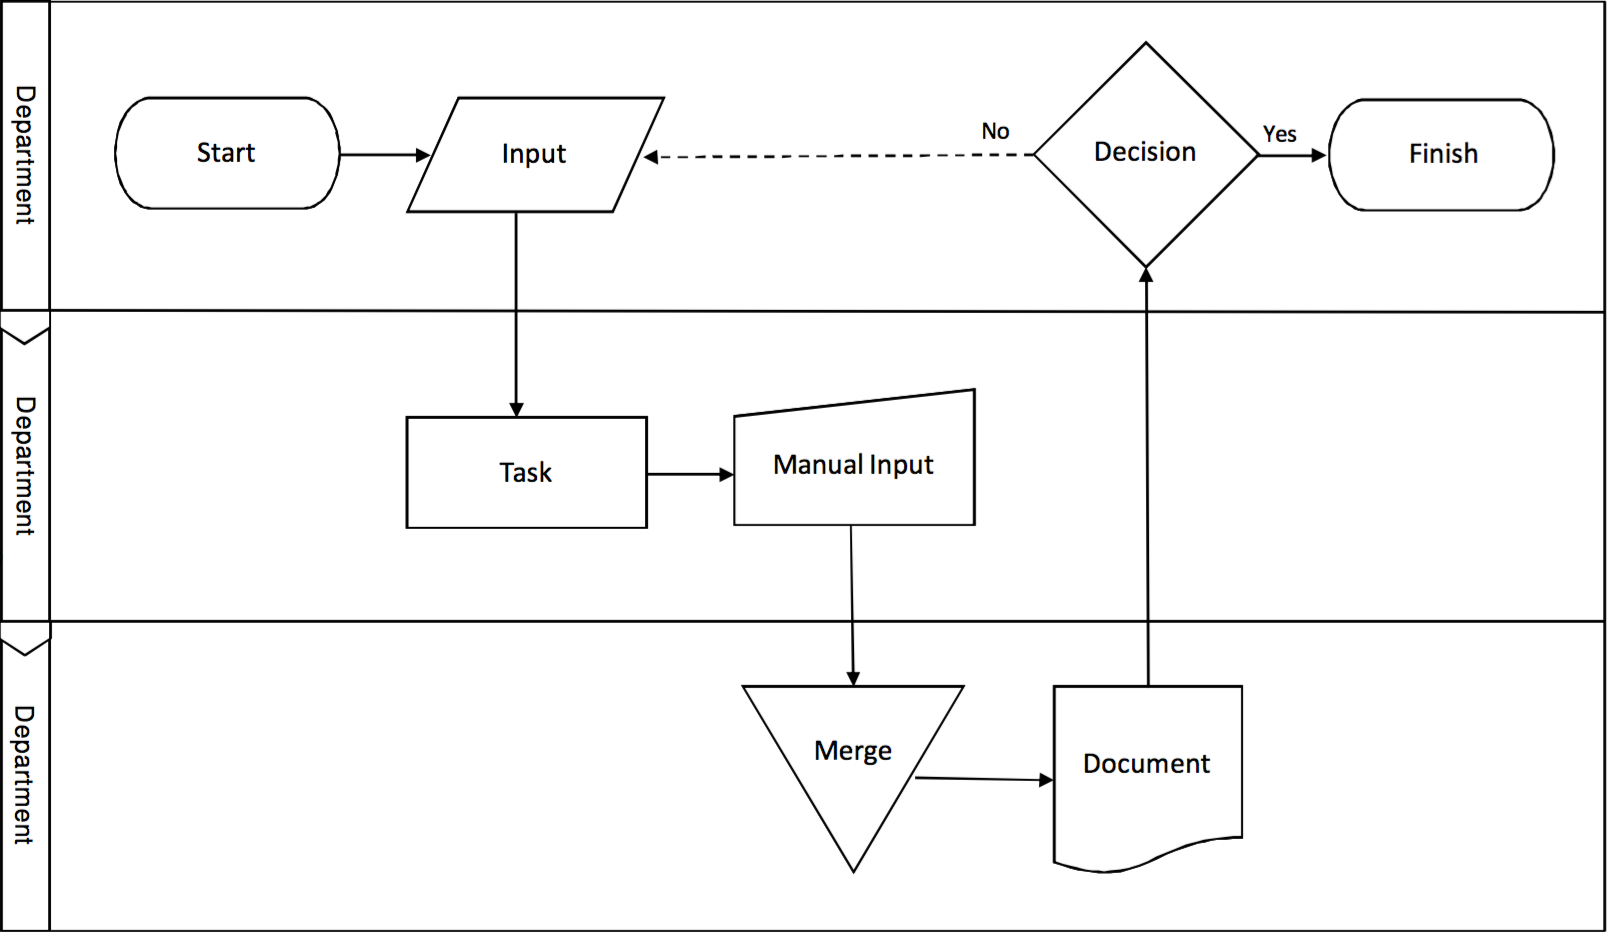
\includegraphics[width=\textwidth]{swimlanes}
	\end{center}
\end{frame}

\begin{frame}{Activity}
	\begin{itemize}
		\item In \textbf{groups of 2-3}
		\item \textbf{Draw} a flowchart for \textbf{logging into Facebook}
		\item Draw your flowchart using \textbf{pen and paper}
		\item Include at least two swimlanes: \textbf{the user's browser/device} and \textbf{the Facebook server}
		\item Take a \textbf{photo} of your flowchart and post it on \textbf{Slack}
	\end{itemize}
\end{frame}

\begin{frame}{Software for drawing flowcharts}
	\pause Intended for drawing flowcharts:
	\begin{itemize}
		\item Gliffy \url{https://www.gliffy.com}
		\item LucidChart
		\item Microsoft Visio
	\end{itemize}
	\pause Can draw flowcharts:
	\begin{itemize}
		\item Microsoft PowerPoint
		\item Google Docs
	\end{itemize}
	\pause If you're desperate:
	\begin{itemize}
		\item Any drawing package (Inkscape, Adobe Illustrator, Apple Keynote, ...)
		\item MS Paint
	\end{itemize}
\end{frame}


\part{Pseudocode}
\frame{\partpage}

\begin{frame}{Pseudocode}
	\pause Flowcharts are useful, but...
	\begin{itemize}
		\pause\item Can be time-consuming to draw
		\pause\item Do not reflect structured programming concepts well
	\end{itemize}
	\pause \textbf{Pseudocode} expresses an algorithm in a way that looks more like a structured program
\end{frame}

\begin{frame}{Pseudocode example}
	\begin{algorithmic}
		\State \textbf{print} ``How old are you?''
		\State \textbf{read} $age$
		\If{$age < 13$}
			\State \textbf{print} ``You are a child''
		\ElsIf{$age < 18$}
			\State \textbf{print} ``You are a teenager''
		\Else
			\State \textbf{print} ``You are an adult''
		\EndIf
	\end{algorithmic}
\end{frame}

\begin{frame}{Pseudocode example}
	\begin{columns}
		\begin{column}{0.6\textwidth}
			\begin{algorithmic}
				\State $sum \gets 0$ \Comment{initialisation}
				\For{$i$ in $1, \dots, 9$}
					\State $sum \gets sum + i$
				\EndFor
				\State \textbf{print} $sum$ \Comment{print the result}
			\end{algorithmic}
		\end{column}
	\end{columns}
\end{frame}

\begin{frame}{Pseudocode example}
	\begin{columns}
		\begin{column}{0.6\textwidth}
			\begin{algorithmic}
				\State $a \gets 1$ \Comment{initialisation}
				\While{$a < 100$}
					\State $a \gets a \times 2$
				\EndWhile
				\State \textbf{print} $a$ \Comment{print the result}
			\end{algorithmic}
		\end{column}
	\end{columns}
\end{frame}

\begin{frame}{Formatting pseudocode}
	\begin{itemize}
		\pause\item Pseudocode is a \textbf{communication tool}, not a \textbf{programming language}
		\pause\item Important: \textbf{clear}, \textbf{concise}, \textbf{unambiguous}, \textbf{consistent}
		\pause\item \textbf{Not} important: adhering to a strict set of style guidelines,
			ensuring direct translatability to your chosen programming language
	\end{itemize}
\end{frame}

\begin{frame}{Level of abstraction}
	\pause Whether working with flowcharts or pseudocode, choose your \textbf{level of abstraction} carefully
\end{frame}

\begin{frame}{Level of abstraction: Good}
	\begin{algorithmic}
		\State Fill kettle
		\State Turn kettle on
		\State Put instant coffee in mug
		\If{sugar wanted}
			\State Add sugar
		\EndIf
		\State Wait for kettle to boil
		\If{milk wanted}
			\State Pour water to $\frac45$ full
			\State Add milk
		\Else
			\State Fill mug with water
		\EndIf
		\State Stir
	\end{algorithmic}
\end{frame}

\begin{frame}{Level of abstraction: Not so good}
	\begin{algorithmic}
		\State Position kettle beneath tap
		\State Turn tap on
		\While{water is below halfway point}
			\State Wait
		\EndWhile
		\State Turn tap off
		\State Place kettle on base
		\State Press power button
		\State ...
	\end{algorithmic}
\end{frame}

\begin{frame}{Level of abstraction: Silly}
	\begin{algorithmic}
		\State Place right palm on kettle handle
		\State Bend fingers on right hand
		\State Lift arm upwards
		\While{tap spout is not directly above kettle}
			\State Move arm to the right
		\EndWhile
		\State Place left palm on tap handle
		\State Bend fingers on left hand
		\State Rotate left hand
		\State ...
	\end{algorithmic}
\end{frame}

\begin{frame}{Level of abstraction: also silly}
	\begin{algorithmic}
		\State Make a cup of coffee
	\end{algorithmic}
\end{frame}

\begin{frame}{Activity}
	A number guessing game: The computer chooses a number between 1 and 20 at random.
	The player guesses a number.
	The computer says whether the guessed number is ``too high'', ``too low'' or ``correct''.
	The game ends when the correct number is guessed, or after 5 incorrect guesses.

	\begin{itemize}
		\item In \textbf{groups of 2-3}
		\item \textbf{Write} pseudocode for the number guessing game
		\item \textbf{Post} your pseudocode on Slack
	\end{itemize}
\end{frame}

\begin{frame}{Activity}
	\begin{itemize}
		\item In \textbf{groups of 2-3}
		\item \textbf{Choose} an algorithm from one of the following:
			\begin{itemize}
				\item Lego Robot Olympiad
				\item COMP120 Tinkering Graphics
				\item COMP150 Game Development Project
			\end{itemize}
		\item \textbf{Express} the algorithm as a flowchart \textbf{and}
		\item \textbf{Express} the algorithm as pseudocode
		\item \textbf{Post} both your flowchart and your pseudocode on Slack
	\end{itemize}
\end{frame}


\begin{frame}{Worksheet B}
	\begin{itemize}
		\item Flowcharts and pseudocode
		\item Due in class \textbf{next Tuesday}
	\end{itemize}
\end{frame}

\end{document}
